%----------------------------------------------------------------------------------------
%   PACKAGES AND DOCUMENT CONFIGURATIONS
%----------------------------------------------------------------------------------------

\documentclass[12pt]{article}
\usepackage[english]{babel}
\usepackage[utf8]{inputenc}
\usepackage{float}

\usepackage{graphicx,epstopdf}   %for embedding images and for conveting eps to pdf
\usepackage{subfig}              %for sub images
\usepackage[margin=1in,includefoot]{geometry}	%changes the margins of report to 1 in
\usepackage{lscape}

\usepackage{rotating}   %used for rotating figures
\usepackage[automake,nonumberlist]{glossaries}    %To use glossary
\usepackage{varwidth}
\usepackage{multicol}   %for making columns
\usepackage{amsmath}
\usepackage{appendix}
\usepackage{pdfpages}
\usepackage{empheq}

\usepackage[framed, numbered]{matlab-prettifier}    %to import matlab code

%----------------------------------------------------------------------------------------
%   Acronym/Glossary
%----------------------------------------------------------------------------------------
\makeglossaries
\loadglsentries{glossary}

%----------------------------------------------------------------------------------------
%   Document Start
%----------------------------------------------------------------------------------------

\begin{document}

\begin{titlepage}

\newcommand{\HRule}{\rule{\linewidth}{0.5mm}} % Defines a new command for the horizontal lines, change thickness here

\center % Center everything on the page
 
%----------------------------------------------------------------------------------------
%   HEADING SECTIONS
%----------------------------------------------------------------------------------------

\textsc{\LARGE MSE 480 Manufacturing Systems}\\[1.5cm] % Org Name
\textsc{\Large }\\[0.5cm] % course name
\textsc{\large }\\[0.5cm] % course title

%----------------------------------------------------------------------------------------
%   TITLE SECTION
%----------------------------------------------------------------------------------------

\HRule \\[0.4cm]
{ \huge \bfseries Lab 3: Robotics 2 - Prelab}\\[0.4cm] % Title of report
\HRule \\[1.5cm]
 
%----------------------------------------------------------------------------------------
%   AUTHOR SECTION
%----------------------------------------------------------------------------------------

\begin{minipage}{0.4\textwidth}
    \begin{flushleft} \large
        \emph{Authors:}\\
        Parshant \textsc{Bombhi}\\
        Klark \textsc{Li}
    \end{flushleft}
\end{minipage}
\hfill
\begin{minipage}{0.4\textwidth}
    \begin{flushright} \large
        \emph{Student ID:} \\
        301255126\\
        301276715
    \end{flushright}
\end{minipage}
\vspace{10mm}
%----------------------------------------------------------------------------------------
%   DATE SECTION
%----------------------------------------------------------------------------------------

{\large \today}\\[2cm] % Date, change the \today to a set date if you want to be precise

%----------------------------------------------------------------------------------------
%   LOGO SECTION
%----------------------------------------------------------------------------------------


\includegraphics[scale=2.0]{MSE-Logo.jpg}\\[1cm] %logo
%----------------------------------------------------------------------------------------

\vfill % Fill the rest of the page with whitespace

\end{titlepage}

%----------------------------------------------------------------------------------------
%   Table of Contents/Table of Figures
%----------------------------------------------------------------------------------------
\pagenumbering{roman} %sets numbering of page to roman
\tableofcontents	%makes table of contents
\addcontentsline{toc}{section}{\numberline{}Table Of Contents}	%adds TOC to TOC

\listoffigures
\addcontentsline{toc}{section}{\numberline{}List of Figures}	%adds list of figures to table of contents

 \listoftables
 \addcontentsline{toc}{section}{\numberline{}List of Tables}

\lstlistoflistings
\addcontentsline{toc}{section}{\numberline{}Listings}

% \printglossary
% \addcontentsline{toc}{section}{\numberline{}Glossary}	%adds glossary to table of contents
\pagebreak
%----------------------------------------------------------------------------------------
%   Main Body
%----------------------------------------------------------------------------------------
\setcounter{page}{1}	%resets the page numbering
\pagenumbering{arabic}	%sets numbering of page to arabic
\setlength{\parskip}{1em}

\section{Introduction}
In this prelab we were to find a inverse kinematics solution to a AL5D robot. We used the coordinate frames assigned in figure \ref{fig:frames} and used the position of the end effector to calculate the angles of the joints.

\begin{figure}[H]
    \centering
    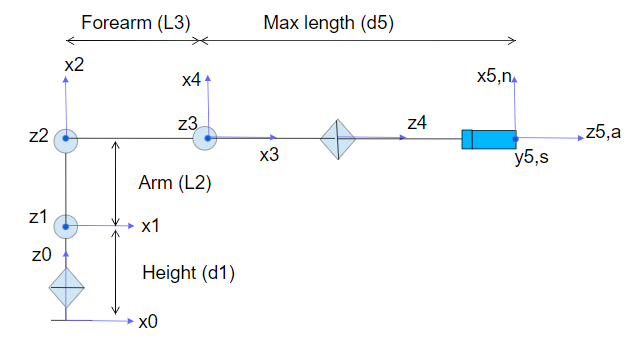
\includegraphics[width=0.8\textwidth]{frames.png}
    \caption{Schematic Diagram of AL5D with Coordinate Frames Assigned}
    \label{fig:frames}
\end{figure}
\noindent
\textbf{Case 1:}\\
\[
T_{0t} =
\begin{bmatrix}
         0 & 0 & 1 & 28.58\\
         0 & -1 & 0 & 0\\
         1 & 0 & 0 & 20.8\\
         0 & 0 & 0 & 1
\end{bmatrix}
\]
\textbf{Case 2:}\\
\[
T_{0t} =
\begin{bmatrix}
         1 & 0 & 0 & 15\\
         0 & -1 & 0 & 5\\
         0 & 0 & -1 & 10\\
         0 & 0 & 0 & 1
\end{bmatrix}
\]
\textbf{Case 3:}\\
\[
T_{0t} =
\begin{bmatrix}
         1 & 0 & 0 & 15\\
         0 & -1 & 0 & 5\\
         0 & 0 & -1 & 1\\
         0 & 0 & 0 & 1
\end{bmatrix}
\]
\textbf{Case 4:}\\
\[
T_{0t} =
\begin{bmatrix}
         1 & 0 & 0 & 15\\
         0 & -1 & 0 & -5\\
         0 & 0 & -1 & 5\\
         0 & 0 & 0 & 1
\end{bmatrix}
\]
The lengths of the arms were given as:
\begin{align*}
    d_1 &= 6.193 cm\\
    L_2 &= 14.605 cm\\
    L_3 &= 18.733 cm\\
    d_5 &= 9.843 cm\\
\end{align*}
\pagebreak
\section{Inverse Kinematics}
We can sub-divide the homogeneous transformation matrix, $T_{0t}$, into components of the orientation and position matrix.
\[
T_{0t} =
\begin{bmatrix}
         R_0^n & P_0^n\\
         0 & 1 \\
\end{bmatrix}
 = 
\begin{bmatrix}
         n & s & a & P_0^n\\
         0 & 0 & 0 & 1\\
\end{bmatrix}
\]
Using the equations provided in class for the spherical wrist we can find $\theta_1$.
\begin{align}
    d_c &= P_0^n - d_5*a\nonumber\\
    \begin{bmatrix}
         d_{cx}\\
         d_{cy}\\
         d_{cz}
\end{bmatrix}
&= 
    \begin{bmatrix}
         P_{x}-d_5*a_1\\
         P_{y}-d_5*a_2\\
         P_{z}-d_5*a_3\nonumber
\end{bmatrix}
\end{align}
We can then use the parameters found to calculate $\theta_1$
\begin{align}
    \theta_1 = tan^{-1}\bigg(\frac{d_{cy}}{d_{cx}}\bigg)
\end{align}
Next we can find $\theta_3$
\begin{align}
    sin(\theta_3) &= \frac{(d_{cz}-d_1)^2+d_{cx}^2+d_{cy}^2-L_2^2-L_3^2}{2L_2L_3}\nonumber\\
    cos(\theta_3) &= \sqrt{(1-(sin(\theta_3))}\nonumber\\
    \theta_3 &= tan^{-1}\bigg(\frac{sin(\theta_3)}{cos(\theta_3)}\bigg)
\end{align}
$\theta_2$ can be found by first finding intermediate matrices A and B:
\begin{align}
    A&=\begin{bmatrix}
             L_2+(L_3*sin(\theta_3)) & L_3*cos(\theta_3)\\
             L_3*cos(\theta_3) & -L_2-(L_3*sin(\theta_3))
    \end{bmatrix}\nonumber\\
    B&=\begin{bmatrix}
             d_{cz}-d_1 & \sqrt(d_{cx}^2+d_{cy}^2)
    \end{bmatrix}\nonumber
\end{align}
Then by dividing the two matrices we get the cosine and sine of the angle. This in turn can be used to find $\theta_2$
\begin{align}
    \begin{bmatrix}
             cos(\theta_2)\\
             sin(\theta_2)
    \end{bmatrix}
    = \frac{A}{B}\nonumber\\
    \theta_2=tan^{-1}\bigg(\frac{sin(\theta_2)}{cos(\theta_2)}\bigg)
\end{align}
Finally we can find $\theta_4$ and $\theta_5$ by:
\begin{align*}
    A_{01} &= 
    \begin{bmatrix}
          cos(\theta_1) & 0 & sin(\theta_1)\\
          sin(\theta_1) & 0 & -cos(\theta_1)\\
          0 & 1 & 0
    \end{bmatrix}\\
    A_{12} &=
    \begin{bmatrix}
             -sin(\theta_2) & -cos(\theta_2) & 0\\
             cos(\theta_2) & -sin(\theta_2) & 0 \\
              0 & 0 & 1
    \end{bmatrix}\\
    A_{23} &=
    \begin{bmatrix}
             sin(\theta_3) & cos(\theta_3) & 0\\
             -cos(\theta_3) & sin(\theta_3) & 0 \\
              0 & 0 & 1
    \end{bmatrix}\\
    R_{03}&=A_{01}A_{12}A_{23}\\
    R_{3t}&=R_{03}*R_{0t}\\
\end{align*}
\begin{align}
    cos(\theta_4) = R_{3t}(1,3)\nonumber\\
    sin(\theta_4) = R_{3t}(2,3)\nonumber\\
    cos(\theta_5) = R_{3t}(3,2)\nonumber\\
    sin(\theta_5) = R_{3t}(3,1)\nonumber\\
    \theta_4 = tan^{-1}\bigg(\frac{sin(\theta_4)}{cos(\theta_4)}\bigg)\\
    \theta_5 = tan^{-1}\bigg(\frac{sin(\theta_5)}{cos(\theta_5)}\bigg)
\end{align}
\pagebreak
\section{Results}


By inputting the rotation angles given for each joint we found transformation matrix for each case.\\

From the resultant transformation matrix we can find the rotation and orientation of the end effector.

We can further solve for the angle of rotation of the end effector by taking the four quadrant inverse tangent of the rotation matrix. Thus giving us:
% Table generated by Excel2LaTeX from sheet 'Sheet1'
\begin{table}[htbp]
  \centering
  \caption{Add caption}
    \begin{tabular}{|p{3.5em}|rrrrr|}
    \hline
    \multicolumn{1}{|r|}{} & \multicolumn{1}{l}{\theta_1} & \multicolumn{1}{l}{\theta_2} & \multicolumn{1}{l}{\theta_3} & \multicolumn{1}{l}{\theta_4} & \multicolumn{1}{l|}{\theta_5} \\
    \hline
    Case 1 & 0     & -0.0157 & 0.0218 & -0.0061 & 0 \\
    Case 2 & 18.4349 & 11.493 & -13.518 & -87.974 & 18.4349 \\
    Case 3 & 18.4349 & 0.2261 & -32.327 & -57.899 & 18.4349 \\
    Case 4 & -18.435 & 7.8519 & -25.946 & -71.906 & -18.435 \\
    \hline
    \end{tabular}%
  \label{tab:addlabel}%
\end{table}%

\pagebreak

\appendix
\section{Matlab Code}
\lstinputlisting[style=Matlab-editor, basicstyle=\mlttfamily\scriptsize, caption={Matlab Code for Joint Angles}]{MSE480_Robotics2_Prelab.m}
\end{document}
              
            